\documentclass[%
 sor,
 jor,
 amsmath,amssymb,
 reprint,
]{revtex4-2}
\usepackage{ulem}
\usepackage{graphicx}
\usepackage{xcolor}
\usepackage{siunitx}
\usepackage{dcolumn}
\usepackage{bm}
\usepackage{amsmath, amssymb, amsfonts}
\usepackage{placeins}
\usepackage{float}
\usepackage{pgfplots}
\pgfplotsset{compat=1.17}



\begin{document}

\title{Experiment 7\\Lee's Method}

\author{Aumshree P. Shah\\20231059}
\altaffiliation{\color{red}aumshree.pinkalbenshah@students.iiserpune.ac.in}
\date{\today}

\begin{abstract}
\centering
In this experiment the thermal conductivity of a bad conductor is measured. 
\end{abstract}

\maketitle

\section{Theory and Procedure}
\subsection{Apparatus}
\small
\begin{minipage}{0.48\textwidth}
\begin{itemize}
\item Lee’s Apparatus \item Bad conductor discs \item Two thermometers \item Boiler and Induction 
\end{itemize}
\end{minipage}
\begin{minipage}{0.48\textwidth}
\begin{itemize}
	\item Stop watch \item Weighing balance \item Vernier Caliper \item Screw gauge
\end{itemize}
\end{minipage}
\subsection{Theory}
Fourier’s law of heat conductance gives the rate of transfer of heat between two objects at temperatures ${T_1}$ and ${T_2}$ connected by a conductor with conductivity $k$, uniform cross-sectional area $A$, and length $l$ as 
\[
\frac{\Delta Q}{\Delta t} = k\,A\,l\,\left({T_2}-{T_1}\right).
\]
This equation governs the rate of heat transfer from disc ${D_2}$ to disc ${D_1}$ (the bottom and top discs of Lee’s apparatus, respectively).\\

The instantaneous rate at which a warm body loses heat to its surroundings is given by Newton’s law of cooling,
\[
\frac{dT}{dt} = -b\,(T-T_a),
\]
where $T_a$ is the ambient temperature. This law governs the rate at which disc ${D_1}$ cools in the second half of the experiment.
If $m$ is the mass of disc ${D_1}$ and $s$ is the specific heat of its material, then the rate at which heat is lost by the disc is 
\[
\frac{\Delta Q_1}{\Delta t} = m\,s\,\frac{dT_1}{dt}.
\]\\

In the steady state achieved in the first half of the experiment, the heat supplied by the steam is balanced by the cooling of disc ${D_1}$. Combining the two heat transfer equations gives the heat balance
\begin{equation}
m\,s\,\frac{dT}{dt} = k\,A\,l\,\left({T_2}-{T_1}\right).
\end{equation}
The value of $\frac{dT}{dt}$ for disc ${D_1}$ can be determined from the cooling curve obtained in the second part of the experiment. As an approximation, a single value of $\frac{dT}{dt}$, calculated at ${T_1}$ during the cooling of disc ${D_1}$ from ${T_1} + \SI{10}{\celsius}$ to ${T_1} - \SI{7}{\celsius}$, is used.
From the known value $s=\SI{0.380}{J\,g^{-1}\,K^{-1}}$ for brass, the conductivity $k$ can be determined.
Note that if the two thermometers do not initially show the same reading, the temperature difference ${T_2}-{T_1}$ must be corrected by the quantity ${T'}$ determined at the beginning of the experiment.

\subsection{Procedure}
\begin{enumerate}
    \item Fill the boiler with water to nearly half and heat it to produce steam. In the meantime, weigh the disc ${D_1}$ on which the apparatus rests.
    \item Measure the diameter of specimen disc $d$ with a vernier calliper and its thickness using a screw gauge at several points, and determine the mean thickness.
    \item Clamp the glass specimen between the base disk ${D_2}$ of the steam jacket and the auxiliary brass disc ${D_1}$. Insert the thermometers (either mercury thermometer or thermocouples) in the two brass disks ${D_1}$ and ${D_2}$.
    \item Check if they show the same readings at room temperature. If not, note the difference $T'$.
    \item Connect the boiler outlet with the inlet of the steam chamber by a rubber tube. Continue passing steam until the two brass disks reach a steady temperature. Note down the temperatures $T_1$ and $T_2$ of the two discs.
    \item The second part of the experiment involves the determination of the cooling rate of disc ${D_1}$ alone. Remove the sample disc. Heat the disc ${D_1}$ directly by the steam chamber until its temperature is about $T_1 + \SI{10}{\celsius}$.
    \item Remove the steam chamber and place the insulating disk on it. Record the temperature of the brass disc at half-minute intervals. Continue until the temperature falls to about $T_1 - \SI{7}{\celsius}$.
\end{enumerate}



\subsubsection{Precautions}
\begin{itemize}
	\item Use thermal gloves while working with the instrument.
	\item Make sure all the contacts are proper.
	\item 
\end{itemize}



\section{Observations}
\noindent Least count of weighing scale:   \uline{1 g}  \\
Least count of thermometer:  \uline{ 0.5 $\si{\celsius}$ }\\
Least count of vernier calliper:  \uline{$10^{-4}$ m } \\
Least count of screw gauge:  \uline{$10^{-5}$ m } \\

\noindent $T'=0$\\
\noindent$M_{D_1} = $ 905 g



\begin{table}[h]
\centering
\begin{tabular}{|c|c|c|}
    \hline
    Material & Diameter $(10^{-5} \si{\meter})$  & Length (cm) \\
    \hline
    Glass	& 410-376-376-376-376 & 11.80\\
    Ebonite 	& 203-119-197-201-199 & 11.20-11.30\\
    Rubber 	& 331 & 9.88-10.00\\
    \hline
\end{tabular}
\caption{Data taken on 19 Mar 2025, the different observations are seperated by '-'.}

\end{table}


\begin{table}[h]
\centering
\begin{tabular}{|c|c|c|}
    \hline
    Material & $T_1 (\si{\celsius})$  &  $T_1 (\si{\celsius})$ \\
    \hline
    Glass	& 86.0 & 95.0\\
    Ebonite 	& 76.0& 94.5\\
    Rubber 	& 84.0& 95.0 \\
    \hline
\end{tabular}
\caption{Data taken on 19 Mar 2025, the different observations are seperated by '-'.}
\end{table}
\begin{table}[H]
\label{tab:}
\centering
  \begin{tabular}{|c|c|}
	  \hline
	  $T~\si{\celsius}$   &  $t$ (sec)\\
	  \hline
 91.5   &7 \\
	  90.5 & 8 \\
	  89.5 & 11 \\
	  88.5 & 11 \\
	  87.5 & - \\
	  86.5 & - \\
	  85.5 & 16 \\
	  84.5 & 17 \\
	  83.5 & - \\
	  82.5 & 21 \\
	  81.5 & 21 \\
	  80.5 & 19 \\
	  79.5 & 23 \\
	  78.5 & 22 \\
	  77.5 & 22 \\
	  \hline
  \end{tabular}
  \caption{Data taken on 21 Mar 2025, the rate of cooling for $D_2$ where $T$ is the mean of floor and celing of the one degree temperature range.}
\end{table}

\section{Uncertainties and Error Sources}
\subsection{Measurement Uncertainties}
\begin{itemize}
	\item \textbf{Weight Measurements:}
    \item \textbf{Length Measurements:} 
    \item \textbf{Temperature Measurements:} Uncertainty of $\pm 0.05$ \si{\kelvin} due to instrument resolution.
\end{itemize}
\subsection{Random Errors}
\begin{itemize}
	\item STUFF
\end{itemize}

\subsection{Systematic Errors}
\begin{itemize}
	\item STUFF
\end{itemize}



\section{Calculation and Error Analysis}
\subsection{Error Propagation}
Using Equation-1 we get: k = ms l A T ˙T2 -T1 From the length, temperature and mass uncertainty, the error to k will travel using the formula for error propagation as: ENTER A BOOK ERROR PROPER HERE 
\subsection{Calculation}
We calculate the value of $\alpha$ of all data points and their uncertainity from hte above formul,  we get (Refer to [3] for calculations):

\begin{table}[h]
\centering
\begin{tabular}{ccc}
\hline
Material & $\alpha$ (\si{1/\degreeCelsius}) \\
\hline
Aluminium & $(2.33 \pm 0.02) \times 10^{-5}$ \\
Aluminium & $(2.32\pm 0.02) \times 10^{-5}$ \\
Brass & $(1.90\pm 0.02) \times 10^{-5}$ \\
Brass & $(1.88\pm 0.02) \times 10^{-5}$ \\
Brass & $(1.92\pm 0.02 \times 10^{-5}$ \\
Copper & $(1.67\pm 0.02) \times 10^{-5}$ \\
Copper & $(1.68\pm 0.02) \times 10^{-5}$ \\
Steel & $(1.61\pm 0.02) \times 10^{-5}$ \\
Steel & $(1.71\pm 0.02) \times 10^{-5}$ \\
Steel & $(1.68\pm 0.02) \times 10^{-5}$ \\

\hline


\end{tabular}
\caption{Calculated expansion coefficients}
\end{table}

\section{Result}
	    The final expansion values by weighted average$^{[1]}$ are:\\
\begin{table}[h]
\centering
\renewcommand{\arraystretch}{1.2}
\begin{tabular}{|c|c|c|c|}
\hline
\textbf{Material} & \textbf{$\alpha$ (1/\textdegree C)} & \textbf{Uncertainty (1/\textdegree C)} & \(\chi^2_\nu\) \\
\hline
Aluminium & \(2.328\times10^{-5}\) & \(6.1\times10^{-8}\) & 0.15 \\
Brass     & \(1.90\times10^{-5}\) & \(1.73\times10^{-7}\) & 2.70 \\
Copper    & \(1.674\times10^{-5}\) & \(3.60\times10^{-8}\) & 0.10 \\
Steel     & \(1.67\times10^{-5}\) & \(3.07\times10^{-7}\) & 11.14 \\
\hline
\end{tabular}
\end{table}





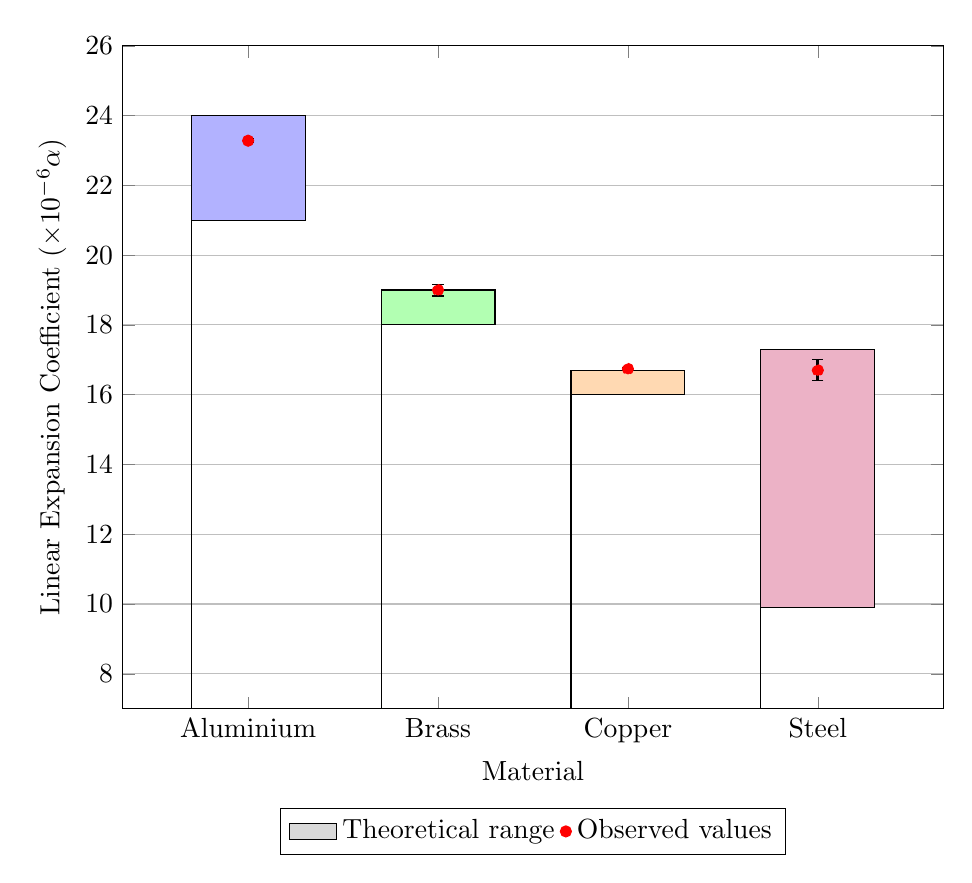
\begin{tikzpicture}
  % Set up the axis with custom dimensions, white background,
  % and y-axis starting at 7 for better visibility of error bars.
  \begin{axis}[
      width=12cm,
      height=10cm,              % Increased height for clear error bar visibility
      xlabel={Material},
      ylabel={Linear Expansion Coefficient ($\times 10^{-6} \alpha$)},
      xtick={1,2,3,4},
      xticklabels={Aluminium, Brass, Copper, Steel},
      ymin=7, ymax=26,          % y-axis range from 7 to 26
      ymajorgrids=true,
      axis background/.style={fill=white}, % Set the background to white instead of pink
      legend style={at={(0.5,-0.15)},anchor=north,legend columns=2},
  ]

  % Add legend entries:
  % - Theoretical range (displayed as a colored rectangle)
  % - Observed value with error bars (red dot with black error bars)
  \addlegendimage{area legend, fill=gray!30, draw=black}
  \addlegendentry{Theoretical range}
  \addlegendimage{only marks, mark=*, mark options={red}}
  \addlegendentry{Observed values}

  %-------------------------------
  % Plot theoretical ranges as colored rectangles
  % Each rectangle represents the range for the material.
  % The width of 0.6 units (from x-0.3 to x+0.3) centers the rectangle at the xtick.
  
  % Aluminium: theoretical range [21, 24]
  \addplot [draw=black, fill=blue!30] coordinates {
    (1-0.3,21) % Bottom left corner
    (1+0.3,21) % Bottom right corner
    (1+0.3,24) % Top right corner
    (1-0.3,24) % Top left corner
  } \closedcycle; % Close the cycle to form a rectangle

  % Brass: theoretical range [18, 19]
  \addplot [draw=black, fill=green!30] coordinates {
    (2-0.3,18)
    (2+0.3,18)
    (2+0.3,19)
    (2-0.3,19)
  } \closedcycle;

  % Copper: theoretical range [16, 16.7]
  \addplot [draw=black, fill=orange!30] coordinates {
    (3-0.3,16)
    (3+0.3,16)
    (3+0.3,16.7)
    (3-0.3,16.7)
  } \closedcycle;

  % Steel: theoretical range [9.9, 17.3]
  \addplot [draw=black, fill=purple!30] coordinates {
    (4-0.3,9.9)
    (4+0.3,9.9)
    (4+0.3,17.3)
    (4-0.3,17.3)
  } \closedcycle;

  %-------------------------------
  % Plot observed values with error bars:
  % The observed values are marked with red dots.
  % The error bars are drawn with a solid, dark black line and the caps are filled black.
  \addplot+[
      only marks,
      mark=*,
      mark options={red}, % Red dot for the observed value
      error bars/.cd,
      y dir=both,        % Error bars in both upward and downward directions
      y explicit,        % Use the explicit error value provided
      error bar style={color=black, line width=1pt, solid}, % Solid, dark black error bars
 %     error mark options={draw=black, fill=black, solid} % Filled black error bar caps
  ] coordinates {
      (1,23.28) +- (0,0.06) % Aluminium observed value with ±0.2 error
  };

  \addplot+[
      only marks,
      mark=*,
      mark options={red},
      error bars/.cd,
      y dir=both,
      y explicit,
      error bar style={color=black, line width=1pt, solid},
  ] coordinates {
      (2,19.0) +- (0,0.17) % Brass observed value with ±0.2 error
  };

  \addplot+[
      only marks,
      mark=*,
      mark options={red},
      error bars/.cd,
      y dir=both,
      y explicit,
      error bar style={color=black, line width=1pt, solid},
  ] coordinates {
      (3,16.74) +- (0,0.04) % Copper observed value with ±0.2 error
  };

  \addplot+[
      only marks,
      mark=*,
      mark options={red},
      error bars/.cd,
      y dir=both,
      y explicit,
      error bar style={color=black, line width=1pt, solid},
  ] coordinates {
      (4,16.7) +- (0,0.3) % Steel observed value with ±0.2 error
  };

  \end{axis}
\end{tikzpicture}












\noindent\rule{\linewidth}{0.4pt}

\newpage
\appendix
\section{Theoretical Values}
The expected values of $\alpha$ in \si{\per\celsius} are [4]:
\[
\begin{split}
\alpha_{\text{Steel}} &= (0.99 - 1.73) \times 10^{-5}\\
\alpha_{\text{Brass}} &= (1.8-1.9) \times 10^{-5}\\
\alpha_{\text{Aluminium}} &= (2.1 - 2.4) \times 10^{-5}\\
\alpha_{\text{Copper}} &= (1.6 - 1.67) \times 10^{-5}
\end{split}
\]

\section{Temperature of rod}\label{rodtemp}
The temperature of rod measured with the application of thermal paste is found to be ranging between $98~\si{\celsius}-99~\si{\celsius}$ (measured on 19 Mar 2025)




\end{document}
